\section{Outlier Removal}

Function \ccc{CGAL::remove_outliers()} deletes a user-specified fraction of outliers from an input point set. More specifically, it sorts the input points in increasing order of average squared distances to their $k$ nearest neighbors and deletes the points with largest value.

% % Insert image remove_outliers.jpg/eps
% \begin{center}
%     % Image
%     \begin{ccTexOnly}
%         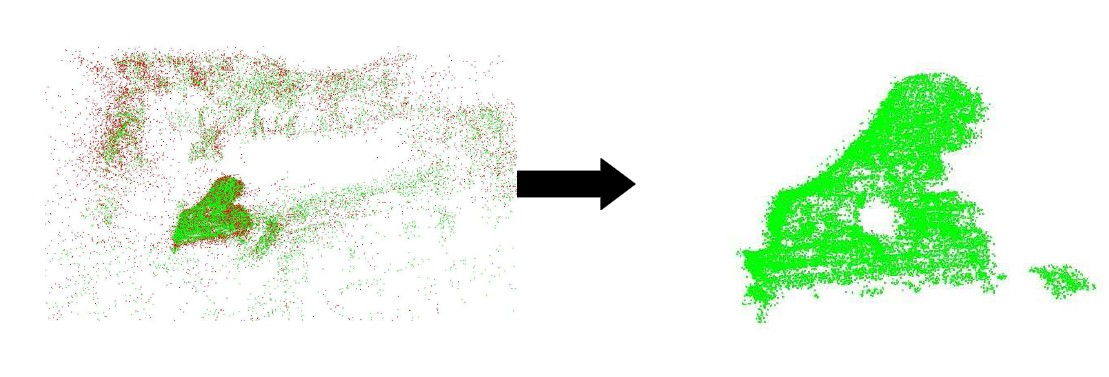
\includegraphics[width=1.0\textwidth]{Point_set_processing_3/remove_outliers} % omit .eps suffix
%     \end{ccTexOnly}
%     \begin{ccHtmlOnly}
%         <img style="max-width: 90%;" border=0 src="./remove_outliers.jpg"><P>
%     \end{ccHtmlOnly}
%     % Title
%     \begin{figure}[h]
%         \caption{Outlier removal}
%         \label{Point_set_processing_3-fig-remove_outliers}
%     \end{figure}
% \end{center}

\ccExample

The following example reads a point set and removes 5\% of the points. It uses the \ccc{CGAL::Dereference_property_map<Point_3>} property map (optional as it is the default position property map of all functions in this component.)
\ccIncludeExampleCode{Point_set_processing_3/remove_outliers_example.cpp}
